On va supposer par l'absurde qu'à partir des quatre triangles isométriques du départ, on puisse les diviser de telle manière à ne plus avoir de triangles isométriques. Pour ceci, on commence par remarquer que si l'on divise un triangle rectangle en $2$ comme dans l'énoncé, les nouveaux triangles rectangles formés sont semblables à celui de départ car ils ont chacun un angle en commun avec lui. Ainsi, comme les quatre triangles de départ sont isométriques et donc semblables, tous les triangles formés après certaines étapes seront toujours semblables.

Pour se débarrasser des triangles isométriques, il est nécessaire de couper au moins $3$ des quatre triangles. On forme alors $6$ nouveaux triangles rectangles, qui forment deux groupes $\mathcal{A}$ et $\mathcal{B}$ de $3$ triangles isométriques. Nécessairement, on doit ensuite couper au moins deux des trois triangles de chaque groupe pour former quatre groupes de $2$ triangles isométriques. Mais on peut en fait construire un groupe de $4$ triangles isométriques car un des triangles formé en coupant un triangle de $\mathcal{A}$ est isométrique à un des triangles formé en coupant un triangle de $\mathcal{B}$, comme le montre bien la figure. Ainsi, on se retrouve nécessairement de nouveau avec $4$ triangles rectangles isométriques. On est alors obligés de répéter toutes les étapes de division jusque là, et comme on ne peut faire qu'un nombre fini de coupes, on ne pourra jamais s'arranger pour ne plus avoir de triangles isométriques.

\begin{center}
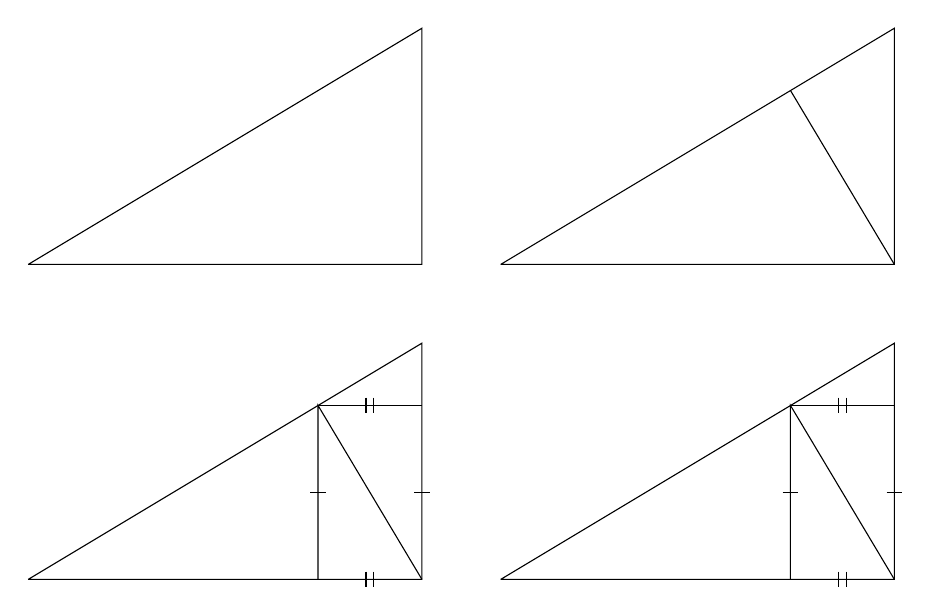
\begin{tikzpicture}
\begin{scope}[shift={(0,0)}]
\draw (0,0) -- (5,0) -- (5,3) -- (0,0);
\draw (5,0) -- (3.68,2.21) -- (3.68,0);
\draw (3.68,2.21) -- (5,2.21);
\draw (4.29,2.31) -- (4.29,2.11);
\draw (4.39,2.31) -- (4.39,2.11);
\draw (4.29,0.1) -- (4.29,-0.1);
\draw (4.39,0.1) -- (4.39,-0.1);
\draw (3.58,1.1) -- (3.78,1.1);
\draw (4.9,1.1) -- (5.1,1.1);
\end{scope}
\begin{scope}[shift={(6,0)}]
\draw (0,0) -- (5,0) -- (5,3) -- (0,0);
\draw (5,0) -- (3.68,2.21) -- (3.68,0);
\draw (3.68,2.21) -- (5,2.21);
\draw (4.29,2.31) -- (4.29,2.11);
\draw (4.39,2.31) -- (4.39,2.11);
\draw (4.29,0.1) -- (4.29,-0.1);
\draw (4.39,0.1) -- (4.39,-0.1);
\draw (3.58,1.1) -- (3.78,1.1);
\draw (4.9,1.1) -- (5.1,1.1);
\end{scope}
\begin{scope}[shift={(0,4)}]
\draw (0,0) -- (5,0) -- (5,3) -- (0,0);
\end{scope}
\begin{scope}[shift={(6,4)}]
\draw (0,0) -- (5,0) -- (5,3) -- (0,0);
\draw (5,0) -- (3.68,2.21);
\end{scope}
\end{tikzpicture}
\end{center}